\documentclass[a4paper]{article}

\usepackage[english]{babel}
\usepackage[utf8]{inputenc}
\usepackage{amsmath}
\usepackage{graphicx}
\usepackage{color}
\usepackage{float}
\usepackage{listings}
\definecolor{keywords}{RGB}{255,0,90}
\definecolor{comments}{RGB}{0,0,113}
\definecolor{red}{RGB}{160,0,0}
\definecolor{green}{RGB}{0,150,0}
\definecolor{codegreen}{rgb}{0,0.6,0}
\definecolor{codegray}{rgb}{0.5,0.5,0.5}
\definecolor{codepurple}{rgb}{0.58,0,0.82}
\definecolor{backcolour}{rgb}{0.95,0.95,0.92}
\definecolor{brown}{rgb}{0.59, 0.29, 0.0}
\definecolor{beaublue}{rgb}{0.74, 0.83, 0.9}
\definecolor{orange}{rgb}{1.0, 0.5, 0.0}
\definecolor{darkslategray}{rgb}{0.18, 0.31, 0.31}
\definecolor{deepblue}{rgb}{0,0,0.5}
\definecolor{deepred}{rgb}{0.6,0,0}
\definecolor{deepgreen}{rgb}{0,0.5,0}
\definecolor{auburn}{rgb}{0.43, 0.21, 0.1}
\definecolor{bistre}{rgb}{0.24, 0.17, 0.12}
\definecolor{babyblue}{rgb}{0.54, 0.81, 0.94}
\definecolor{ballblue}{rgb}{0.13, 0.67, 0.8}
\lstdefinestyle{myMatlabstyle}{
	language=Matlab,
	backgroundcolor=\color{white},   
	commentstyle=\color{deepgreen},
	keywordstyle=\color{black},
	identifierstyle=\color{black},
	numberstyle=\tiny\color{codegray},
	stringstyle=\color{purple},
	basicstyle=\footnotesize,
	breakatwhitespace=false,         
	breaklines=true,                 
	captionpos=b,                    
	keepspaces=true,                 
	numbers=left,                    
	numbersep=5pt,                  
	showspaces=false,                
	showstringspaces=false,
	showtabs=false,                  
	tabsize=2
}
\lstdefinestyle{myPythonstyle}{
	language=Python, 
	basicstyle=\ttfamily\small, 
	keywordstyle=\color{blue},
	commentstyle=\color{green},
	stringstyle=\color{red},
	showstringspaces=false,
	identifierstyle=\color{black},
}
\lstset{language=Matlab,frame=single}
\lstset{language=Python,frame=single}
\usepackage[colorinlistoftodos]{todonotes}
\usepackage[scale=0.75]{geometry}
	\title{Estimating speech from lip movement}

\author{Jithin D. George, Ronan Keane, Connor Zellmer}

\date{\today}

\begin{document}
\maketitle

\begin{abstract}

\end{abstract}

\section{Introduction and Overview}
\label{sec:introduction}

\begin{figure}[H] 
	\centering
	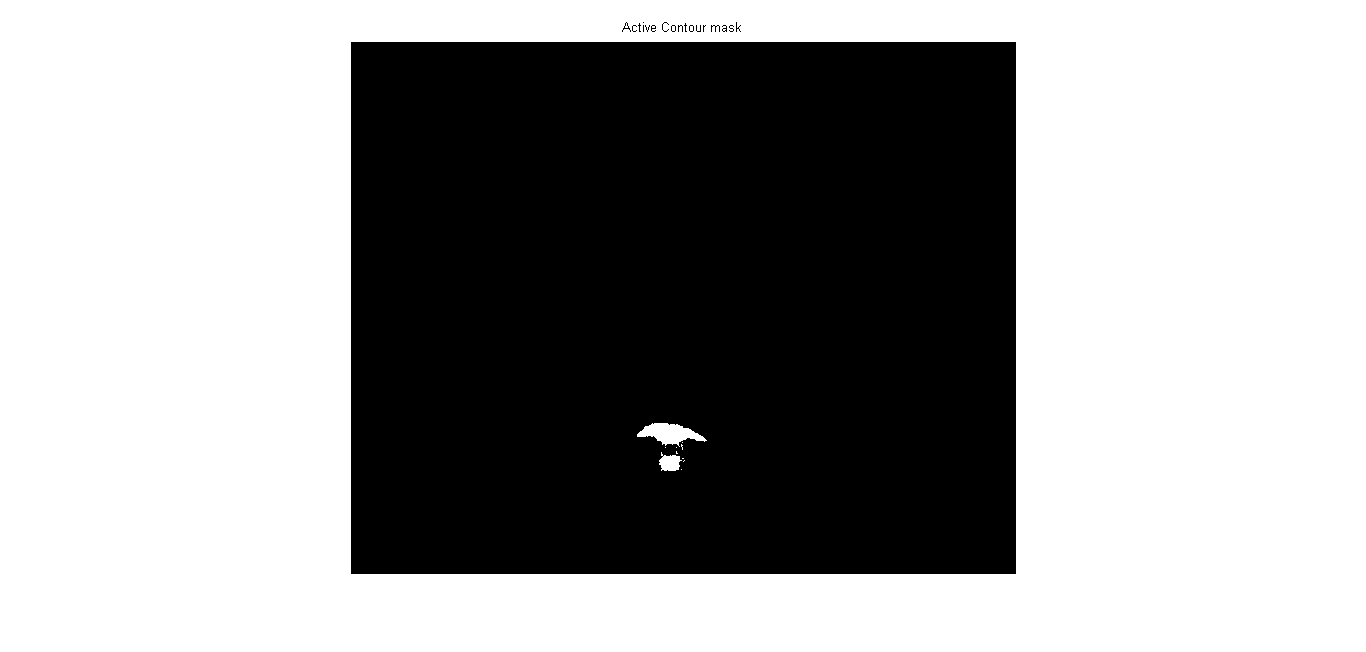
\includegraphics[width=0.7\textwidth]{active}
	\caption{Active Contour}	
\end{figure}

\begin{figure}[H] 
	\centering
	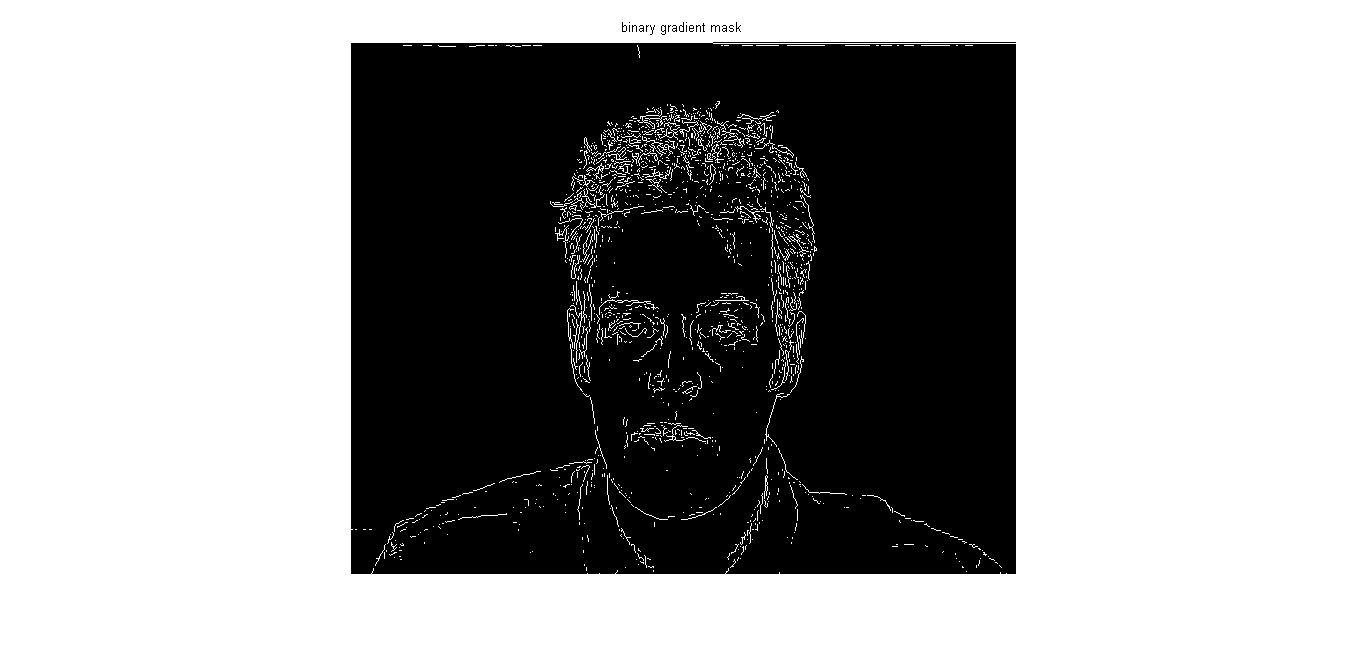
\includegraphics[width=0.7\textwidth]{binary}
	\caption{Binary Gradient}	
\end{figure}
\section{Theoretical Background}
\label{sec:theory}

\section{Hidden Markov Models}

A Markov model involves the transition of a particular state to other states based on transition probabilities. A future state is only depends on the current state and not the states before it. Now, consider that at every state, there would be real world observations. These observations are controlled by the emission probabilities at each state.

For example, if we were to represent the ever changing weather, the states would be sunny, rainy or snowing and the observations would be summer clothes, rain boots or snow shoes. We can see that the emission probabilities for each observation is different depending on the state. To be more clear, the emission probabilities depend on the states.

We look at Hidden Markov Models(HMM). We decide that this is a relevant model because the words spoken are those defined by language and thus occur in specific pattern and not randomly. For example, given the first letter of word 'k', the probability that the next letter is a vowel is much higher than it being a consonant. A machine learning algorithm without this would be as inefficient as the initial Enigma machine in the movie "The Imitation Game". HMMs are very popular in the fields of speech \cite{key-2} and gesture recognition \cite{key-4} \cite{key-5}.

Although HMMs have fascinating problems related to evaluation and learning, our interests are in decoding. We have a sequence of observations and our aim is to estimate the states that created that. The Viterbi algorithm \cite{key-3} gives us the states that maximize the occurrence of the observations. 

So, given the features from the videos, we find the states. The states are the units of words, here chosen to be phonemes. 
\section{Implementation and Development}

\subsection{Extracting Phonemes}

Using the nltk library in Python, we convert every word to its constitutive arpabet phonetics. It gives the following output for the words - f', 'see', 'sea', 'compute', 'comput', 'cat'. Only 'comput' fails because it isn't a real word
\begin{verbatim}
['EH1', 'F']
['S', 'IY1']
['S', 'IY1']
['K', 'AH0', 'M', 'P', 'Y', 'UW1', 'T']
'comput'
['K', 'AE1', 'T']
\end{verbatim}

From the words spoken in our videos, we get a set of 36 unique phonemes. The code for this is shown in using \ref{Ph.py} The 36 unique phonemes are 

\begin{verbatim}
'AA1', 'AE1', 'AH0', 'AH1', 'AO1', 'AW1', 'AY1', 'B', 'CH', 'D', 'DH', 'EH1', 'EY1', 'F', 
 'G', 'IH0', 'IH1', 'IY1', 'JH', 'K', 'L', 'M', 'N', 'OW0', 'OW1', 'P', 'R', 'S', 'T',
  'TH', 'UW0', 'UW1', 'V', 'W', 'Y', 'Z
\end{verbatim}

\section{Jobs}

This section is where we see the stuff to do.

\begin{itemize}
	\item lip tracking using color classification (Ronan)
	\item figures of edge tracking for the report 
	\item Getting the transition probabilities between phonemes (Jithin)
	\item Getting a feature space for each phoneme.
	\subitem Code to extract all the output from the subtitles file. (Extract words and times)
	\subitem Code to guess how to split phonemes for each word 
	\subitem Code to align and crop lips 
	\subitem Code to split aligned lips to match phonemes
	\item Something with nnets.
\end{itemize}

\section{Computational Results}

\section{Summary and Conclusions}

Further step and modifications.



\begin{thebibliography}{1}
	\bibitem{key-1}J. Proctor, S. Brunton and J. N. Kutz, Dynamic mode decomposition with control, arXiv:1409.6358.
	\bibitem{key-2}Rabiner, Lawrence R. "A tutorial on hidden Markov models and selected applications in speech recognition." Proceedings of the IEEE 77.2 (1989): 257-286.	
	\bibitem{key-3}Forney, G. David. "The viterbi algorithm." Proceedings of the IEEE 61.3 (1973): 268-278.
	
	\bibitem{key-4}Yang, Jie, and Yangsheng Xu. Hidden markov model for gesture recognition. No. CMU-RI-TR-94-10. CARNEGIE-MELLON UNIV PITTSBURGH PA ROBOTICS INST, 1994.

	\bibitem{key-5}Starner, Thad E. Visual Recognition of American Sign Language Using Hidden Markov Models. MASSACHUSETTS INST OF TECH CAMBRIDGE DEPT OF BRAIN AND COGNITIVE SCIENCES, 1995.
	

\end{thebibliography}

\newpage

\appendix
%dummy comment inserted by tex2lyx to ensure that this paragraph is not empty




\section{MATLAB Code}

\subsection{Contours.m}
\begin{lstlisting}[style=myMatlabstyle]
obj=VideoReader('vid1.mpg');
vidFrames = read(obj);
numFrames = get(obj,'numberOfFrames');
[mov]= getmovout(vidFrames,numFrames-1);
X=frame2im(mov(50));
A=rgb2gray(X);
mask = zeros(size(A));
mask(400:450,320:400) = 1;
bw = activecontour(A,mask,300);
figure, imshow(bw), title('Active Contour mask');
[~, threshold] = edge(A, 'sobel');
fudgeFactor = .5;
BWs = edge(A,'sobel', threshold * fudgeFactor);
figure, imshow(BWs), title('binary gradient mask');
\end{lstlisting}

\section{Python Code}

\subsection{Phonemes.py}
\label{Ph.py}
\begin{lstlisting}[style=myPythonstyle]
import nltk

arpabet = nltk.corpus.cmudict.dict()

for word in ('f', 'see', 'sea', 'compute', 'comput', 'cat'):
		try:
			print(arpabet[word][0])
		except Exception as e:
			print(e)
\end{lstlisting}
\end{document}